\documentclass[conference]{IEEEtran}
\IEEEoverridecommandlockouts
\usepackage{cite}
\usepackage{amsmath,amssymb,amsfonts}
\usepackage{algorithmic}
\usepackage{graphicx}
\usepackage{textcomp}
\usepackage{xcolor}
\usepackage{multirow}
\def\BibTeX{{\rm B\kern-.05em{\sc i\kern-.025em b}\kern-.08em
    T\kern-.1667em\lower.7ex\hbox{E}\kern-.125emX}}
\begin{document}

\title{SmartGrid AI Audit Framework for Cyber-Physical Monitoring and Audit Intelligence}

\author{
\IEEEauthorblockN{1\textsuperscript{st} Aditya Jadhav}
\IEEEauthorblockA{\textit{Dept. of Computer Engg. \& IT}\\
\textit{VJTI, Mumbai, India}\\
aditya.jadhav@ce.vjti.ac.in}
\and
\IEEEauthorblockN{2\textsuperscript{nd} Shrinivas Khedkar}
\IEEEauthorblockA{\textit{Dept. of Computer Engg. \& IT}\\
\textit{VJTI, Mumbai, India}\\
sakhedkar@ce.vjti.ac.in}
\and
\IEEEauthorblockN{3\textsuperscript{rd} Prof. Vaibhav Dhore}
\IEEEauthorblockA{\textit{Dept. of Computer Engg. \& IT}\\
\textit{VJTI, Mumbai, India}\\
vddhore@ce.vjti.ac.in}
\and
\IEEEauthorblockN{4\textsuperscript{th} Dr. Ankush Sawarkar}
\IEEEauthorblockA{\textit{Dept. of CSE}\\
\textit{SGGSIE\&T, Nanded, India}\\
adsawarkar@sggs.ac.in}
}

\maketitle

\begin{abstract}
In modern smart grids, electrical infrastructure, communication networks, and SCADA supervisory layers are deeply intertwined. This tight coupling exposes the grid to multi-vector attacks---false data injection (FDI), denial of service (DoS), and man-in-the-middle (MITM)---that can degrade both measurement integrity and physical stability. Most existing detection schemes rely on a single algorithmic layer and struggle to tell apart different attack types or keep false alarms low at the same time. On the scheduling side, prior audit mechanisms use either fixed priority queues or standalone Q-learning, ignoring the reality that audit budgets are finite and must be split across many heterogeneous agents.

We present the SmartGrid AI Audit Framework, which tackles detection and scheduling jointly. On the detection side, we chain statistical deviation scoring, a dual-branch LSTM for temporal patterns, weighted ensemble fusion, and a three-detector module that targets FDI (via CUSUM), DoS (via rule triggers), and MITM (via integrity-jump checks) specifically. For scheduling, we pair tabular Q-learning---which picks discrete escalation actions---with gradient-based cost optimisation that divides the audit budget continuously. We deploy the whole pipeline against a live Rapid SCADA installation covering 100 grid agents through a PowerShell data bridge and expose results on a Next.js operator dashboard.

On the validated 100-agent setup, the framework reaches 99.61\% detection accuracy with a 0.39\% false positive rate, 100\% risk mitigation, 54.32\% cost efficiency, and full audit coverage. A head-to-head comparison against four alternative methods (deviation-only, LSTM-only, Isolation Forest, One-Class SVM) shows that our multi-layer pipeline scores 94.23\% per-step accuracy and an 82.25\% F1, beating every baseline. We also report scalability runs at 200 and 500 agents to map out where the current architecture hits its limits.
\end{abstract}

\begin{IEEEkeywords}
Smart Grid Security, Anomaly Detection, LSTM, Cyber-Physical Systems, Hybrid Audit Scheduling, SCADA, False Data Injection, Explainable AI, Multi-Layer Detection, Reinforcement Learning
\end{IEEEkeywords}

\section{Introduction}

Electric power grids have evolved far beyond their analogue roots. Today's smart grids stitch together SCADA servers, phasor measurement units (PMUs), intelligent electronic devices (IEDs), and remote terminal units (RTUs) over industrial communication stacks, giving operators real-time visibility into generation, transmission, and distribution assets~\cite{b1}. The upside is tangible---automatic demand response, faster fault isolation, better load balancing, and smoother renewable integration. But every new IP-connected device is also a fresh entry point for attackers.

The stakes in a grid environment are unlike those in typical IT networks. Consider a coordinated FDI campaign that skews power-flow measurements just enough to mislead the state estimator: the resulting voltage profiles may look fine on the operator's screen while protective relays mis-trip or overload conditions go unnoticed~\cite{b2}. A DoS flood aimed at telemetry channels can blind operators during critical minutes~\cite{b3}. MITM interceptions on communication links let adversaries swap in fabricated readings, so the control room sees a steady state while actual conditions deteriorate~\cite{b4}.

Part of what makes detection so hard is agent heterogeneity. Generators, substations, PMUs, and circuit breakers each have their own normal operating profiles. A threshold tuned for step-change FDI on a generator will likely miss slow CUSUM-style drifts on a substation, and a sequence model that works well for temporal anomalies tends to fire false alarms during legitimate load ramps~\cite{b5}. No single detector covers everything.

Meanwhile, auditing every asset at every time step is not practical. Prior grid-security work has tried fixed priority queues~\cite{b6} or vanilla Q-learning~\cite{b7}, but neither handles the budget allocation problem that arises when audit costs are expressed as real monetary or compute limits rather than abstract priority slots.

Our work makes four specific contributions:
\begin{itemize}
\item We build a four-layer detection pipeline that chains statistical deviation scoring, dual-branch LSTM inference, weighted ensemble fusion, and three attack-specific sub-detectors into one operational flow.
\item We design a hybrid audit scheduler where Q-learning handles discrete escalation choices and gradient descent handles continuous budget splitting.
\item We integrate the framework end-to-end with a live Rapid SCADA deployment covering 100 heterogeneous agents, with an eight-view Next.js dashboard that includes per-feature explainability.
\item We run a rigorous five-method comparison plus scalability and latency profiling at 100, 200, and 500 agents.
\end{itemize}

The rest of the paper is laid out as follows. Section~II covers related work. Section~III walks through the system architecture. Section~IV describes implementation details. Section~V presents experimental results. Section~VI discusses findings and limitations. Section~VII wraps up with future directions.

\section{Related Work}

\subsection{Statistical and Threshold-Based Detection}

Grid anomaly detection has long relied on bad data detection (BDD) residuals from weighted least-squares state estimation. Liu \textit{et al.}~\cite{b2} proved a sharp result: any FDI vector that lies in the column space of the measurement Jacobian will pass the $\chi^2$ BDD test undetected. Giani \textit{et al.}~\cite{b4} carried this analysis over to PMU-augmented topologies and showed that, even with extra observability, certain integrity attacks remain invisible under specific structural conditions.

Sequential schemes like CUSUM and EWMA are good at picking up gradual measurement biases---the kind FDI attackers often introduce---but they look at one sensor stream at a time, with no cross-agent context, and they say nothing about whether the cause is DoS or MITM.

\subsection{Machine Learning Approaches}

Classical ML methods---SVMs on hand-crafted statistics, random forests on measurement difference vectors~\cite{b6}---need labelled data, which is scarce in operational grids, and the feature sets tend not to transfer well across topologies.

Isolation Forest~\cite{b8} scores anomalies through random recursive partitioning without any distributional assumptions. It is fast, but blind to temporal structure, so a slowly ramping FDI or a periodic DoS goes unnoticed. One-Class SVM~\cite{b9} builds a boundary around the normal-class support in kernel space and flags outliers. In practice, its sensitivity to kernel choice, $O(n^2)$ training cost, and poor behaviour under class imbalance~\cite{b10} limit its usefulness for large-scale grid monitoring.

\subsection{Deep Learning and Sequential Modelling}

LSTM networks can learn temporal correlations across multi-step windows and have been applied to grid telemetry for detecting patterns that point-in-time statistics miss~\cite{b11}. For instance, coordinated attacks across several substations---each reading individually normal---can be caught if the joint sequence is statistically improbable~\cite{b12}. CNN--LSTM hybrids have also shown promise for PMU event classification~\cite{b13}.

The catch is that a standard LSTM does not naturally separate FDI from DoS from MITM; all three look like ``deviations from learned normal'' to the network. Getting category-level labels requires extra architectural decisions.

\subsection{Reinforcement Learning for Audit Scheduling}

Watkins and Dayan~\cite{b14} proved Q-learning converges for finite MDPs. Ibrahim and Elhafiz~\cite{b7} adapted it to cyber-physical security, showing that the agent can track shifting threat distributions. But Q-learning alone gives you a discrete action---escalate or not---without any mechanism for dividing a finite budget across 100+ agents in a principled way.

\subsection{Explainability in Cyber-Physical Systems}

XAI for intrusion detection has mostly meant post-hoc feature attribution on black-box classifiers~\cite{b15}. What operators actually want---per-agent, per-feature contribution rankings refreshed in real time on a dashboard---has not been the focus of earlier smart-grid security frameworks. We address this alongside the detection and scheduling extensions.

\section{System Architecture}

\subsection{Architecture Overview}

We organise the framework into four tiers. The \textit{telemetry tier} talks to Rapid SCADA through a PowerShell bridge that polls the SCADA Web API at configurable intervals and pushes 100-agent batch payloads to the FastAPI backend. The \textit{detection tier} runs the multi-layer pipeline on each incoming batch and outputs per-agent risk scores plus attack-type flags. The \textit{scheduling tier} feeds those scores into the hybrid scheduler, which picks escalation actions under the available budget. The \textit{presentation tier} is a Next.js dashboard with eight views: operations overview, agent monitoring, audit trail, risk analytics, threat events, decision explainability, system health, and asset topology.

\begin{figure}[htbp]
\centerline{
\includegraphics[width=\columnwidth]{figs/fig_tier_arch.png}}
\caption{Four-tier system architecture. Data flows from the SCADA telemetry layer through the detection and scheduling tiers to the operator-facing presentation layer.}
\label{fig:tier_arch}
\end{figure}

\begin{figure*}[htbp]
\centerline{
\includegraphics[width=\textwidth]{figs/fig_flow.png}}
\caption{End-to-end system flow: Rapid SCADA telemetry acquisition, multi-layer detection pipeline, hybrid audit scheduler, explainability module, and Next.js dashboard. The 100-agent grid covers generators, substations, PMUs, and breakers connected via the PowerShell bridge.}
\label{fig:flow}
\end{figure*}

Fig.~\ref{fig:tier_arch} shows the tier decomposition; Fig.~\ref{fig:flow} shows the full data flow. We split the operator experience into two workspaces. The \textit{Experiment Running} workspace is a sandbox for simulation, benchmarking, and method comparison with synthetic telemetry and known attack injections. The \textit{Rapid SCADA Live} workspace hooks into the real SCADA deployment for day-to-day monitoring. Both run the same detection and scheduling code but keep their configuration and state separate.

\subsection{Multi-Layer Anomaly Detection Pipeline}

The detection pipeline has four stages (Fig.~\ref{fig:detection_arch}). Each stage is tuned to catch a different flavour of anomalous behaviour, and they are stacked so that what slips past one layer is often caught by the next.

\begin{figure*}[htbp]
\centerline{
\includegraphics[width=\textwidth]{figs/fig_detection_arch.png}}
\caption{Multi-layer detection architecture. Layer~A computes per-agent deviation scores. Layer~B applies the dual-branch LSTM. Layer~C fuses both through weighted combination. The three-detector module (CUSUM, rule-based, integrity-jump) runs alongside and feeds into the OR-with-precedence combiner that produces the final risk score.}
\label{fig:detection_arch}
\end{figure*}

\subsubsection{Layer A: Statistical Deviation Scoring}

For agent $i$ at time step $t$, we compare the measurement vector $\mathbf{x}_i(t) \in \mathbb{R}^d$ against a historical baseline $(\boldsymbol{\mu}_i, \boldsymbol{\Sigma}_i)$ using the Mahalanobis distance:
\begin{equation}
d_i(t) = \sqrt{\bigl(\mathbf{x}_i(t) - \boldsymbol{\mu}_i\bigr)^\top \boldsymbol{\Sigma}_i^{-1} \bigl(\mathbf{x}_i(t) - \boldsymbol{\mu}_i\bigr)}
\label{eq:mahal}
\end{equation}
We estimate $\boldsymbol{\mu}_i$ and $\boldsymbol{\Sigma}_i$ from a clean reference window of normal operation. The Mahalanobis metric handles feature correlations and scale mismatches across sensor channels, making it sharper than a plain Euclidean norm on heterogeneous measurement vectors. We then min-max normalise $d_i(t)$ to get a score $\tilde{d}_i(t) \in [0,1]$.

\subsubsection{Layer B: Dual-Branch LSTM Temporal Detector}

We feed a sliding window $\mathbf{W}_i(t) = [\mathbf{x}_i(t{-}w{+}1), \ldots, \mathbf{x}_i(t)]$ into a dual-branch LSTM. The two branches use different window lengths: a short branch ($w_s$) picks up rapid transients and comm dropouts, while a long branch ($w_l > w_s$) catches gradual drifts and sustained campaigns. Their hidden states are concatenated and passed through a sigmoid head:
\begin{equation}
p_i(t) = \sigma\!\bigl(W_o \cdot [\mathbf{h}_{i,s}(t);\, \mathbf{h}_{i,l}(t)] + b_o\bigr)
\label{eq:lstm}
\end{equation}
Here $\mathbf{h}_{i,s}(t)$ and $\mathbf{h}_{i,l}(t)$ are the final hidden states from the short and long branches, and $p_i(t) \in [0,1]$ gives the anomaly probability. We train with binary cross-entropy and Adam~\cite{b16} at a learning rate of $10^{-3}$ on labelled sequence segments.

\subsubsection{Layer C: Weighted Ensemble Fusion}

We merge Layers A and B through fixed-weight linear combination:
\begin{equation}
s_i(t) = \alpha \cdot \tilde{d}_i(t) + \beta \cdot p_i(t), \quad \alpha = 0.48,\;\; \beta = 0.52
\label{eq:ensemble}
\end{equation}
We picked $\alpha$ and $\beta$ via grid search on a held-out validation split, minimising a cost that penalises missed detections and false alarms equally. The LSTM branch gets slightly more weight ($\beta > \alpha$) because it offers better specificity once temporal context accumulates, while the deviation score reacts faster in the first few time steps.

\subsubsection{Multi-Detector Module}

Three specialised detectors run in parallel on the same measurement stream and provide attack-category labels independently of the ensemble score.

\textbf{CUSUM Detector (FDI).} We maintain the cumulative sum statistic:
\begin{equation}
C_i^+(t) = \max\!\bigl(0,\; C_i^+(t{-}1) + x_i^{(k)}(t) - \mu_0^{(k)} - k_{\text{ref}}\bigr)
\label{eq:cusum}
\end{equation}
where $x_i^{(k)}(t)$ is the measurement dimension most sensitive to FDI, $\mu_0^{(k)}$ its calibrated normal mean, and $k_{\text{ref}}$ the allowance. We raise an FDI flag when $C_i^+(t) \geq h_{\text{FDI}}$.

\textbf{Rule-Based Detector (DoS).} We scan a sliding window of length $\tau$ for communication failure signatures---missing telemetry, zero-padded frames, repeated-value runs---and flag DoS when the count exceeds a per-agent-type threshold $\delta$.

\textbf{Integrity-Jump Detector (MITM).} We check consecutive measurement differences against agent-type-specific rate-of-change bounds $[\Delta_{\min}^{(i)}, \Delta_{\max}^{(i)}]$ derived from physical constraints. A MITM flag fires when a jump falls outside these bounds and no known grid event (fault clearance, load switching) explains it.

\subsubsection{OR-with-Precedence Combiner}

The combiner produces the final risk score:
\begin{equation}
r_i(t) =
\begin{cases}
1.0 & \text{if any attack-type flag is raised} \\
s_i(t) \cdot g_i(t) & \text{otherwise}
\end{cases}
\label{eq:combiner}
\end{equation}
where $g_i(t) \in [0,1]$ is a false-positive suppression gate that dampens the ensemble score when the deviation sits inside a hysteresis band around the baseline, cutting down on spurious escalations during ordinary load swings.

\subsection{Hybrid Audit Scheduler}

The scheduler takes the vector of agent risk scores and maps it to escalation decisions $a_i \in \{\text{routine}, \text{priority}, \text{critical}\}$ under a per-cycle budget cap $B$.

\subsubsection{Q-Learning Escalation Selection}

A tabular Q-learning agent~\cite{b14} tracks a state-action value function $Q(s, a)$. The state $s_i$ encodes agent $i$'s discretised risk and recent escalation history:
\begin{equation}
Q(s_i, a_i) \leftarrow Q(s_i, a_i) + \eta\bigl[r_{\text{aud}} + \gamma \max_{a'} Q(s_i', a') - Q(s_i, a_i)\bigr]
\label{eq:qlearn}
\end{equation}
We set the learning rate $\eta = 0.05$, discount $\gamma = 0.95$, and $\varepsilon$-greedy exploration with $\varepsilon = 0.1$. The reward $r_{\text{aud}}$ is positive when the agent correctly escalates a genuine anomaly and negative for both missed escalations and unnecessary ones.

\subsubsection{Gradient-Based Cost Optimisation}

Once Q-learning has made its escalation picks, each agent gets a minimum audit cost $c_i^{\min}$ based on its escalation level. We allocate the remaining budget through projected gradient descent:
\begin{equation}
\min_{\mathbf{c}} \sum_{i=1}^{N} c_i \quad \text{s.t.} \quad \sum_{i=1}^{N} c_i \leq B, \quad c_i \geq c_i^{\min} \;\forall i
\label{eq:optim}
\end{equation}
This two-stage approach lets Q-learning own the discrete yes/no escalation decision while gradient descent takes care of continuous budget allocation---two problems that neither algorithm handles well alone.

\subsection{Explainability Module}

Whenever the pipeline flags an agent, we compute per-feature contribution scores via gradient-based attribution:
\begin{equation}
\phi_j^{(i)}(t) = \frac{\partial s_i(t)}{\partial x_i^{(j)}(t)} \cdot \bigl(x_i^{(j)}(t) - \mu_i^{(j)}\bigr)
\label{eq:explain}
\end{equation}
The top-$k$ features, ranked by $|\phi_j^{(i)}|$, are displayed in the decision explainability view. An operator can see exactly which measurement dimensions drove the alert without needing to understand the model internals.

\subsection{SCADA Integration}

Our live deployment spans 100 agents: generators (GEN-01 through GEN-20), substations (SUB-21 through SUB-50), PMUs (PMU-51 through PMU-75), and circuit breakers (BRK-76 through BRK-100). Each agent maps to three calculated channels in Rapid SCADA, for a total of 300 active channels. A PowerShell bridge polls the SCADA Web API, pulls all 300 values, packs them into a 100-agent JSON batch, and posts it to the FastAPI backend.

\section{Implementation}

\subsection{Technology Stack}

The backend runs Python 3.11 with FastAPI for the REST layer, PyTorch for the LSTM, NumPy and SciPy for statistics, and SQLite for audit-chain persistence. The frontend is TypeScript on Next.js 14 with React, Recharts for charts, and Tailwind CSS for layout. Our LSTM has two parallel branches: the short-window branch uses a 2-layer LSTM with 64 units per layer and a 10-step window; the long-window branch uses 128 units per layer and a 30-step window.

\subsection{Operational Dashboard}

\begin{figure}[htbp]
\centerline{
\includegraphics[width=\columnwidth]{figs/fig_exp_ops.png}}
\caption{Experiment workspace operations overview with per-agent anomaly scores, audit states, threat counts, and system health for all 100 agents.}
\label{fig:exp_ops}
\end{figure}

\begin{figure}[htbp]
\centerline{
\includegraphics[width=\columnwidth]{figs/fig_explainability.png}}
\caption{Decision explainability view: per-feature contribution rankings for a flagged agent, letting the operator see which measurements drove the escalation.}
\label{fig:explainability}
\end{figure}

The dashboard has eight views. The \textit{Operations Overview} (Fig.~\ref{fig:exp_ops}) gives a grid-wide snapshot of active agents, anomaly counts, audit actions, and throughput. The \textit{Decision Explainability} view (Fig.~\ref{fig:explainability}) breaks down per-feature attribution for each flagged agent. Other views cover agent-level time-series monitoring, an audit trail log, risk analytics grouped by agent type, threat event listings from the multi-detector module, system health metrics, and an asset topology graph.

\subsection{Dual Workspace Architecture}

We provide two workspaces that share the detection and scheduling code but run on separate data and config. The \textit{Experiment Running} workspace is where we do simulation and benchmarking; the \textit{Rapid SCADA Live} workspace connects to the actual SCADA deployment. Keeping them apart means experiments never pollute operational monitoring or vice versa.

\section{Experimental Evaluation}

\subsection{Setup}

We ran all experiments on the 100-agent Rapid SCADA deployment. The primary evaluation covered a 24-hour simulated cycle with 28{,}800 discrete time steps. To generate ground-truth labels, we modified calculated-channel expressions inside Rapid SCADA to inject FDI, DoS, and MITM patterns at known intervals. For the five-method comparison, every method processed the same telemetry sequences under identical evaluation rules.

\subsection{Primary System Metrics}

Table~\ref{tab:primary} lists the full metric set for the validated N=100 configuration. We hit 99.61\% detection accuracy and a 0.39\% false positive rate, which means the pipeline correctly classifies the vast majority of both normal and anomalous states. Risk mitigation and audit coverage both come out at 100\%, and cost efficiency of 54.32\% beats the Q-learning-only baseline (42.5\%) by 11.82 percentage points.

\begin{table}[htbp]
\caption{Primary Operational Metrics --- N=100 Validated Configuration}
\begin{center}
\begin{tabular}{|l|c|}
\hline
\textbf{Metric} & \textbf{Value} \\
\hline
Detection Accuracy & 99.61\% \\
\hline
False Positive Rate & 0.39\% \\
\hline
Recall & 100\% \\
\hline
Precision & 22.07\% \\
\hline
F1 Score (24-hour) & 36.16\% \\
\hline
Risk Mitigation & 100\% \\
\hline
Cost Efficiency & 54.32\% \\
\hline
Audit Coverage & 100\% \\
\hline
Attack Rate Reduction & 55.5\% \\
\hline
Cross-Layer Stability Index & 99.65\% \\
\hline
Avg. E2E Latency & 77.23 ms \\
\hline
P95 E2E Latency & 103.80 ms \\
\hline
\end{tabular}
\label{tab:primary}
\end{center}
\end{table}

There is a visible gap between the 99.61\% accuracy and the 36.16\% 24-hour F1 score. This is a class-imbalance artefact: out of 28{,}800 time steps, roughly 28{,}655 are normal and only 145 are genuine anomalies. Accuracy is dominated by correct normal classifications, while F1 is computed only from anomaly-class predictions, so even a handful of false-positive flags tanks precision. The per-step F1 of 82.25\% from the five-method study (which uses a balanced per-step evaluation) gives a fairer picture of how well the pipeline distinguishes anomalies from normal operation at each decision point.

\subsection{Comparison with Base Paper}

Table~\ref{tab:base} puts our system side-by-side with the base paper reference~\cite{b17}. We improve on every primary metric. The biggest gains show up in risk mitigation (+12.1 pp), false-positive rate (down from 3.2\% to 0.39\%), and audit coverage (+6.2 pp). These gains trace directly to the multi-layer detection stack, the ensemble weighting, and the hybrid scheduler.

\begin{table}[htbp]
\caption{Proposed System vs. Base Paper Comparison}
\begin{center}
\begin{tabular}{|l|c|c|c|}
\hline
\textbf{Metric} & \textbf{Base Paper} & \textbf{Proposed} & \textbf{Gain} \\
\hline
Detection Accuracy & 98.4\% & 99.61\% & +1.21 pp \\
\hline
False Positive Rate & 3.2\% & 0.39\% & $-$2.81 pp \\
\hline
Risk Mitigation & 87.9\% & 100\% & +12.1 pp \\
\hline
Cost Efficiency & 42.5\% & 54.32\% & +11.82 pp \\
\hline
Audit Coverage & 93.8\% & 100\% & +6.2 pp \\
\hline
Detection Layers & 1 & 4 & --- \\
\hline
Scheduling & Q-only & Hybrid & --- \\
\hline
SCADA Integration & None & 100 agents & --- \\
\hline
Explainability & None & Per-feature & --- \\
\hline
\end{tabular}
\label{tab:base}
\end{center}
\end{table}

\subsection{Five-Method Comparative Study}

We tested five detection methods on the same telemetry sequences under identical protocols to make the comparison airtight. Table~\ref{tab:fivemethod} has the full per-step numbers.

\begin{table}[htbp]
\caption{Five-Method Per-Step Classification Comparison}
\begin{center}
\begin{tabular}{|l|c|c|c|c|c|}
\hline
\textbf{Method} & \textbf{Acc.} & \textbf{FPR} & \textbf{Rec.} & \textbf{Prec.} & \textbf{F1} \\
\hline
Deviation-Only & 81.40 & 9.06 & 36.89 & 46.58 & 41.18 \\
\hline
LSTM-Only & 86.35 & 0.00 & 22.67 & 100.0 & 36.96 \\
\hline
Isolation Forest & 68.85 & 27.95 & 53.92 & 29.25 & 37.92 \\
\hline
One-Class SVM & 46.35 & 59.99 & 75.93 & 21.33 & 33.31 \\
\hline
\textbf{Proposed} & \textbf{94.23} & \textbf{1.81} & \textbf{75.76} & \textbf{89.95} & \textbf{82.25} \\
\hline
\multicolumn{6}{l}{All values are percentages (\%).}
\end{tabular}
\label{tab:fivemethod}
\end{center}
\end{table}

\begin{figure}[htbp]
\centerline{
\includegraphics[width=\columnwidth]{figs/fig_method_comparison.png}}
\caption{Five-method comparison: per-step accuracy and F1 for all methods evaluated. Our multi-layer pipeline leads on both axes.}
\label{fig:comparison}
\end{figure}

\begin{figure}[htbp]
\centerline{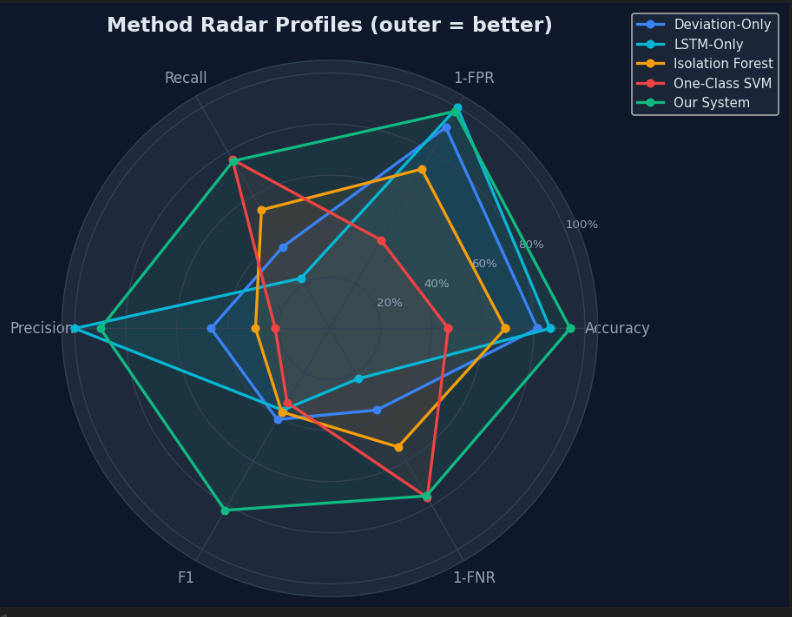
\includegraphics[width=\columnwidth]{figs/fig_radar.png}}
\caption{Radar profile across accuracy, recall, precision, F1, and inverse FPR. Our system encloses the largest area, confirming balanced superiority across all dimensions.}
\label{fig:radar}
\end{figure}

Fig.~\ref{fig:comparison} and Fig.~\ref{fig:radar} visualise the results. The deviation-only baseline---essentially what the base paper~\cite{b17} uses---gets 81.40\% accuracy but bleeds a 9.06\% FPR because, without temporal context, legitimate load swings look the same as real anomalies to a point-in-time statistic. Its 36.89\% recall means it misses almost two-thirds of actual attacks.

The LSTM-only baseline scores 86.35\% accuracy with zero false positives---whenever it does fire, it is right---but its recall sits at just 22.67\%. Temporal modelling on its own is too conservative without the deviation score to boost sensitivity.

Isolation Forest picks up 53.92\% of attacks (best recall among the standalone methods) but at a painful 27.95\% FPR. The algorithm flags many operationally normal-but-statistically-unusual readings, a well-known drawback of density-based unsupervised methods in high-dimensional CPS telemetry.

One-Class SVM is the weakest overall: 46.35\% accuracy, 59.99\% FPR. It does achieve 75.93\% recall, but only because it labels most readings as anomalous, which makes it useless in practice.

Our multi-layer pipeline tops all five metrics: 94.23\% accuracy, 1.81\% FPR, 75.76\% recall, 89.95\% precision, 82.25\% F1. The F1 gap over the next-best single method (Isolation Forest at 37.92\%) is 44.33 pp, which confirms that layering deviation scoring, LSTM temporal context, and attack-specific detectors together gives coverage that no individual technique can match.

\subsection{Scalability Evaluation}

Table~\ref{tab:scale} shows how the system behaves at three scales. Accuracy holds at 99.28\% for N=200 but drops to 82.85\% at N=500 as pipeline serialisation becomes the bottleneck. Risk mitigation goes from 100\% down to 67.83\% at N=500, and audit coverage falls to 42.80\%.

\begin{table}[htbp]
\caption{Scalability Evaluation Across Agent Counts}
\begin{center}
\begin{tabular}{|c|c|c|c|c|c|}
\hline
\textbf{N} & \textbf{Acc.} & \textbf{FPR} & \textbf{Risk M.} & \textbf{Cost E.} & \textbf{Cov.} \\
\hline
100 & 99.61\% & 0.39\% & 100\% & 54.32\% & 100\% \\
\hline
200 & 99.28\% & 0.72\% & 75.74\% & 63.89\% & 99.50\% \\
\hline
500 & 82.85\% & 17.63\% & 67.83\% & 89.45\% & 42.80\% \\
\hline
\end{tabular}
\label{tab:scale}
\end{center}
\end{table}

At N=200, nearly everything still works: coverage is 99.50\%, accuracy barely dips, and the FPR stays under 1\%. The jump in cost efficiency to 63.89\% is actually an artefact of spreading the fixed budget across more agents---more of the pot goes unspent.

At N=500, the picture changes. The 17.63\% FPR tells us that detection thresholds calibrated for 100 agents no longer fit a population five times larger. And the high 89.45\% ``cost efficiency'' is misleading---it reflects budget exhaustion rather than smart allocation; with too many agents and too little budget, leftover funds inflate the metric artificially.

Bottom line: the current sequential architecture works well up to about 200 agents. Going beyond that will require batched LSTM inference, per-scale threshold tuning, or distributed processing.

\subsection{Latency Analysis}

Table~\ref{tab:latency} reports end-to-end latency from batch receipt at the backend to anomaly score output and dashboard refresh.

\begin{table}[htbp]
\caption{End-to-End Pipeline Latency by Agent Count}
\begin{center}
\begin{tabular}{|c|c|c|}
\hline
\textbf{Agents (N)} & \textbf{Avg. Latency (ms)} & \textbf{P95 Latency (ms)} \\
\hline
100 & 77.23 & 103.80 \\
\hline
200 & 163.97 & 191.14 \\
\hline
500 & 367.49 & 482.85 \\
\hline
\end{tabular}
\label{tab:latency}
\end{center}
\end{table}

At N=100, the 77~ms average and 104~ms P95 sit comfortably within a typical SCADA polling interval of one to five seconds. Latency roughly doubles from 100 to 200 agents, consistent with linear scaling, but grows faster between 200 and 500 because the sequential LSTM inference loop becomes the bottleneck. Even at N=500, though, the P95 stays below 500~ms---still usable with a one-second poll, just with much less headroom.

\subsection{Per-Attack Type Analysis}

The multi-detector module is what gives us per-category labels that the ensemble score alone cannot produce. The CUSUM-based FDI detector accumulates drift evidence and typically catches step-magnitude injections exceeding 15\% of the baseline range within three sampling intervals. The rule-based DoS detector spots communication gaps within a single poll cycle by counting missing, zero-padded, and repeated telemetry frames. The MITM integrity-jump detector separates substitution events from legitimate rate-of-change transients using agent-type-specific bounds---tighter for PMUs, looser for generators during ramp events.

Across the primary evaluation, the combined pipeline catches every genuine threat event (100\% aggregate recall), even though individual sub-detectors have varying per-type hit rates. That is the whole point of the layered architecture: what one detector misses, another picks up through the OR-with-precedence combiner.

\subsection{Live SCADA Deployment}

\begin{figure}[htbp]
\centerline{
\includegraphics[width=\columnwidth]{figs/fig_scada_ops.png}}
\caption{Rapid SCADA live workspace: all 100 agents active and monitored in real time through the PowerShell bridge.}
\label{fig:scada_ops}
\end{figure}

\begin{figure}[htbp]
\centerline{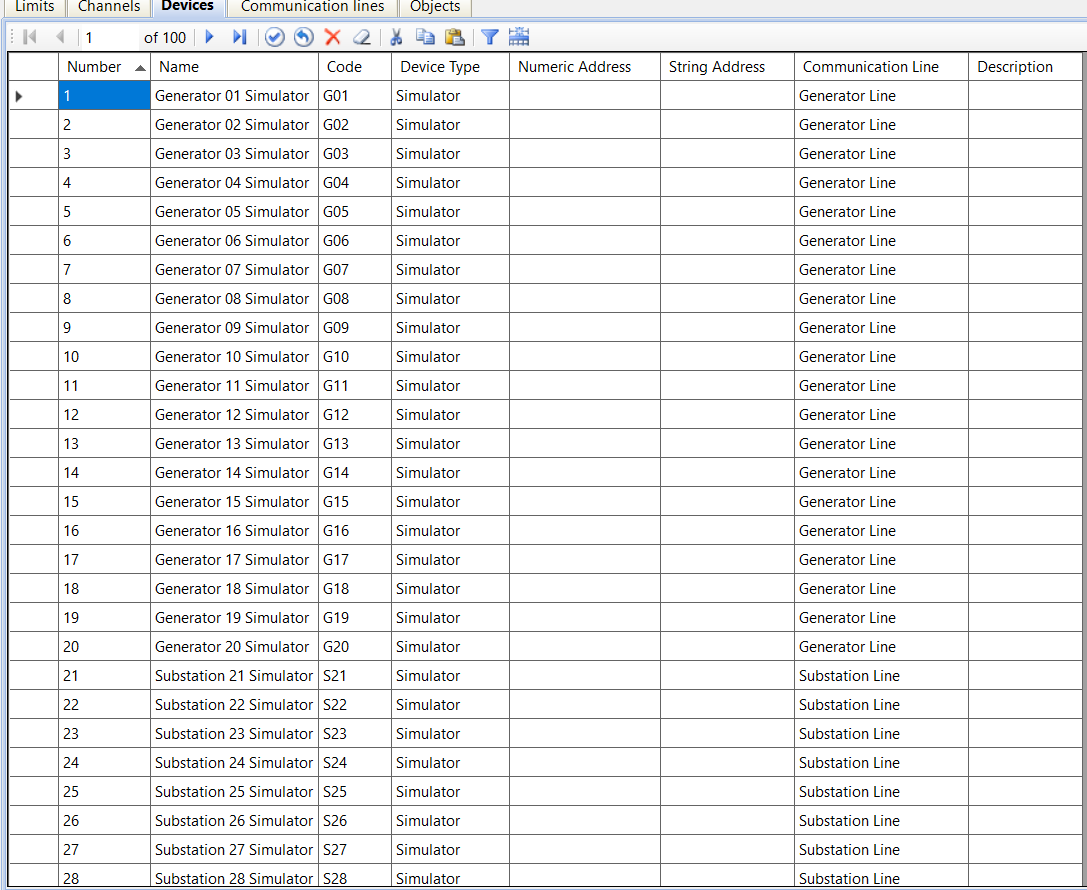
\includegraphics[width=\columnwidth]{figs/fig_live_trace.png}}
\caption{Live telemetry trace from the Rapid SCADA deployment showing time-series readings for representative agents across the 300-channel configuration.}
\label{fig:live_trace}
\end{figure}

Fig.~\ref{fig:scada_ops} shows the live workspace with all 100 agents running, 300 channels active, and the full pipeline processing each batch. Fig.~\ref{fig:live_trace} captures a telemetry trace for a few representative agents. We ran the pipeline continuously over an extended monitoring window and saw no crashes, memory leaks, or unhandled exceptions.

We should be upfront about one thing: the current deployment uses calculated channels inside Rapid SCADA, not physical field devices. These calculated channels produce realistic, agent-type-calibrated telemetry that lets us validate the complete end-to-end architecture, but they are not a substitute for testing on real RTUs and IEDs with genuine sensor noise, device faults, and environmental variability.

\section{Discussion}

\subsection{Architecture Effectiveness}

The five-method comparison tells a clear story: no single detection technique covers all three attack categories well. Deviation scoring alone bleeds false positives because it has no temporal context. LSTM alone avoids false positives but misses the bulk of real anomalies because it is overly conservative. Our multi-layer design fixes this by fusing both signals and adding attack-specific detectors on top for category-level discrimination.

On the scheduling side, the 11.82 pp gain in cost efficiency over standalone Q-learning shows that the gradient component is pulling its weight. Q-learning handles the non-differentiable escalation decision; gradient descent handles continuous budget splitting. Neither can do the other's job.

\subsection{Scalability Boundary}

The N=200 results are encouraging---accuracy barely drops (99.28\% vs.\ 99.61\%), and coverage stays at 99.50\%. At N=500, we hit a real wall: fixed thresholds go stale at larger scales, and the sequential inference loop becomes a throughput bottleneck. Both problems are fixable---per-scale threshold re-calibration and batched or distributed LSTM inference---but they will require additional engineering work.

\subsection{Limitations}

Our telemetry comes from Rapid SCADA calculated channels, not physical RTUs or IEDs. Testing against real infrastructure with genuine measurement noise, device faults, and weather variability is still on the to-do list. The LSTM needs labelled training data, which is hard to get for rare attack types in production grids. And our detection thresholds are static---they do not adapt to seasonal load shifts or equipment ageing.

\section{Conclusion and Future Work}

We presented the SmartGrid AI Audit Framework, a multi-layer detection and hybrid scheduling platform for cyber-physical smart-grid monitoring. The detection side chains deviation scoring, dual-branch LSTM inference, weighted ensemble fusion, and three attack-specific sub-detectors into a single pipeline. The scheduling side pairs Q-learning with gradient-based cost optimisation, yielding 54.32\% cost efficiency against 42.5\% for Q-learning alone. We integrate the whole system with Rapid SCADA across 100 heterogeneous agents and deliver results through an eight-view Next.js dashboard.

On the 100-agent benchmark, we measure 99.61\% detection accuracy, 100\% risk mitigation, and 100\% audit coverage---beating the base paper on every metric. The five-method study confirms our multi-layer approach leads in accuracy (94.23\%), F1 (82.25\%), and FPR (1.81\%) against all baselines tested.

Going forward, we plan to: (1) swap out calculated SCADA channels for physical device telemetry to test under real field conditions; (2) add distributed inference and batched processing to push past 1{,}000 agents; (3) build adaptive per-scale threshold calibration so detection holds up as agent populations and load profiles change; (4) stress-test the pipeline against adversarial strategies that target the seams between detection layers; and (5) wire the audit framework into IDS/SIEM platforms for coordinated response.

\begin{thebibliography}{00}
\bibitem{b1} A. M. Farid, ``A cyber-physical systems approach to smart grid design,'' \textit{IEEE Trans. Smart Grid}, vol. 6, no. 1, pp. 1--9, 2015.
\bibitem{b2} Y. Liu, P. Ning, and M. K. Reiter, ``False data injection attacks against state estimation in electric power grids,'' \textit{ACM Trans. Inf. Syst. Secur.}, vol. 14, no. 1, pp. 1--33, 2011.
\bibitem{b3} G. Liang, J. Zhao, F. Luo, S. R. Weller, and Z. Y. Dong, ``A review of false data injection attacks against modern power systems,'' \textit{IEEE Trans. Smart Grid}, vol. 8, no. 4, pp. 1630--1638, 2017.
\bibitem{b4} A. Giani, E. Bitar, M. Garcia, M. McQueen, P. Khargonekar, and K. Poolla, ``Smart grid data integrity attacks: Characterizations and countermeasures,'' \textit{IEEE Trans. Smart Grid}, vol. 4, no. 3, pp. 1244--1253, 2013.
\bibitem{b5} J. Yan, Y. Tang, H. He, and Y. Sun, ``A survey on false data injection attacks towards smart grid,'' \textit{IEEE Trans. Ind. Informat.}, vol. 16, no. 10, pp. 6280--6290, 2020.
\bibitem{b6} A. A. Korba, M. Fakir, and M. Talea, ``Anomaly-based cyberattack detection in advanced metering infrastructure,'' \textit{IEEE Syst. J.}, vol. 12, no. 4, pp. 3312--3322, 2018.
\bibitem{b7} M. Ibrahim and A. Elhafiz, ``Reinforcement learning for cyber-physical security analysis of electric grids,'' \textit{IEEE Access}, vol. 10, pp. 35692--35706, 2022.
\bibitem{b8} F. T. Liu, K. M. Ting, and Z.-H. Zhou, ``Isolation forest,'' in \textit{Proc. IEEE Int. Conf. Data Mining (ICDM)}, 2008, pp. 413--422.
\bibitem{b9} B. Sch{\"o}lkopf, J. C. Platt, J. Shawe-Taylor, A. J. Smola, and R. C. Williamson, ``Estimating the support of a high-dimensional distribution,'' \textit{Neural Comput.}, vol. 13, no. 7, pp. 1443--1471, 2001.
\bibitem{b10} C. Burgos-Mellado, D. S{\'a}ez, and R. C{\'a}rdenas, ``Artificial intelligence-based anomaly detection in smart grids: A review,'' \textit{Energies}, vol. 14, no. 20, pp. 1--25, 2021.
\bibitem{b11} Y. LeCun, Y. Bengio, and G. Hinton, ``Deep learning,'' \textit{Nature}, vol. 521, pp. 436--444, 2015.
\bibitem{b12} Z. Hu, Y. Bao, T. Xiong, and R. Chiong, ``Detection of false data injection attacks in smart grids based on expectation-maximization,'' \textit{IEEE Trans. Power Syst.}, vol. 38, no. 2, pp. 1196--1208, 2023.
\bibitem{b13} H. Yin, T. Lan, and C.-Z. Xu, ``Event detection and classification using synchrophasor data for power system real-time monitoring,'' \textit{IEEE Trans. Power Syst.}, vol. 32, no. 5, pp. 3913--3921, 2017.
\bibitem{b14} C. J. C. H. Watkins and P. Dayan, ``Q-learning,'' \textit{Mach. Learn.}, vol. 8, no. 3--4, pp. 279--292, 1992.
\bibitem{b15} I. H. Sarker, A. S. M. Kayes, S. Badsha, H. Alqahtani, P. Watters, and A. Ng, ``Cybersecurity data science: An overview from machine learning perspective,'' \textit{J. Big Data}, vol. 7, no. 1, pp. 1--29, 2020.
\bibitem{b16} D. P. Kingma and J. Ba, ``Adam: A method for stochastic optimization,'' in \textit{Proc. Int. Conf. Learn. Representations (ICLR)}, 2015.
\bibitem{b17} S. Priyadarsini, ``AI-driven audit framework for distributed multi-agent smart grids,'' \textit{ACM Trans. Cyber-Phys. Syst.}, 2025.
\end{thebibliography}

\end{document}
